% Header
\renewcommand\evenpagerightmark{{\scshape\small Chapter 7}}
\renewcommand\oddpageleftmark{{\scshape\small Summary and outlook}}

\hyphenation{}

\chapter[Summary and outlooks]{Summary and outlook}
\label{chapt7}

	\section{Summary}
	\label{chapt7:sec:summary}
	
	The upgrade of the \acf{LHC} towards the \acf{HL-LHC} began in 2018 with the start of the \acf{LS2}. The aim is to increase the luminosity of the accelerator to boost its discovery potential for new physics beyond the \acf{SM} in particle physics. Many extensions to the SM feature \acf{HSCPs}, where, in the context of the \acf{CMS}, the muon system could play an important to identify such new particles. An increase in instantaneous luminosity will lead to an increase of the background noise and of the irradiation levels to which the detectors will be subjected. A first issue in the CMS Muon upgrade is the fact that the muon system needs to be certified for the HL-LHC period. Next to this, the muon system will be extended through the installation of new chambers, including also Resistive Plate Chambers (RPCs), in the region closest to the beam line. The goal is to ensure the best quality possible of the muon trigger by mitigating the background effects and increasing the redundancy of the system (muon tracking might also benefit from this). The upgrade will also take place at the level of the Link-Board system connecting the \acf{FEE} of CMS RPCs to the trigger processor to improve its robustness and finally take profit of the real time resolution of chambers of the order of \SI{1}{ns}. The CMS RPC upgrade comprises quite an extensive and exciting research program. The collaboration converged towards the solutions that will be adopted in the perspective of HL-LHC. Even though the consolidation of the present CMS RPC infrastructure and the certification of the new technologies that will complete the redundancy of the muon system are still ongoing, the future of the experiment from the RPC point of view is now clear. To reach this point, my contribution during the preliminary phase of tests between 2012 and 2015 has been decisive in two parts: (i) the consolidation of the present detectors, and (ii) in the selection of the FEEs that will equip the improved RPCs (iRPCs). At every step, I played an important role in setting up the experiments but also in gathering and analysing the data.
	
	The certification of the resulting technologies, adapted for the needs of CMS in the RE3/1 and RE4/1 regions of the muon endcaps, is being performed at the \acf{GIF++} where an irradiation bunker along a muon beam had been built. The facility featured a \SI{14}{TBq} Cesium source. The purpose of this new facility was to conduct various long-term studies in the perspective of the HL-LHC. The prototypes for the improved CMS chambers are trapezoidal double-gap RPCs featuring \acf{HPL} electrodes of \SI{1.4}{mm} and gas gaps of the same thickness. The reduction of the gap thickness was motivated by the lower gain of such detectors at similar electric fields. The read-out PCB consists of 96 longitudinal strips with a pitch ranging from \SI{4}{mm} at the narrow end to \SI{8}{mm} at the wide end. This design defines the baseline of what will be installed in CMS in the future.\\
	My first contribution to the CMS Upgrade was the testing of two selected potential FEE technologies: (i) a low-noise preamplifier using SiGe technology developed at INFN Tor Vergata, and (ii) FEEs based on the PETIROC ASIC also featuring SiGe technology developed by the OMEGA Collaboration and used for timing applications. To limit the ageing of the detectors installed in the challenging region near the beam line, more sensitive electronics operated at lower threshold values (\SI{10}{fC} instead of the current \SI{140}{fC}) will help reducing the gain of the detector and, hence, the related charge deposition.\\
	At two occasions, the INFN preamplifier has been tested and compared to the current CMS FEEs. In a first experiment, the preamplifier was directly connected to four read-out strips of a spare CMS RPC, and the output signal was digitized by the use of a discriminator. The preamplifier was operated with a charge threshold as low as \SI{3}{fC} and showed a working voltage shift of \SI{475}{V} with respect to the RPC operated with the current CMS electronics. To improve the comparison of the INFN technology with the CMS FEB, a FEB without preamplifier was designed to connect and operate the preamplifier. This enabled a direct comparison between the new, low-noise preamplifier, and the current one used by CMS. The electronics were again mounted on spare CMS RPCs to repeat the previous experiment. The shift in working voltage observed reached \SI{410}{V} at a threshold of \SI{5}{fC}, consistent with the first result obtained.\\
	The FEEs developed by OMEGA were tested on a spare CMS RPC gap from the RE4 production. For comparison purposes, the spare gap used was mounted into an RPC case, and the detector was operated in single gap mode with the CMS FEB. The results showed that the HARDROC2 could provide a reduction of the working voltage in single gap mode of almost \SI{500}{V} at charge sensitivity of \SI{121.4}{fC}, comparable to the threshold of the CMS FEEs set at \SI{146}{fC}, while keeping noise levels below \SIrate{0.1}. This technology had also already been certified for other experiments using detectors such as scintillators and RPCs. Finally, it had the advantage of proposing a 2D read-out that would greatly improve the spatial resolution of the detectors in the radial direction. Taking profit of the good time resolution of the electronics of the order of \SI{100}{ps}, the strips of the iRPCs will be read-out from both ends to reach a spatial resolution of \SI{2}{cm} along the strips that would greatly profit to the particle tracking in CMS.\\
	Several prototypes have been assembled and are used to test the CMS RPCROC FEEs derived from the PETIROC technology and the INFN Tor Vergata alternative that was adapted to the requirements of the CMS RPC. For comparison purposes, cosmic tests without irradiation have been conducted on the iRPC prototypes using the current CMS FEBs. The detector reached its working voltage at \SIerror{7383}{70}{V} with an efficiency near 97\% when operated at a threshold of \SI{133}{fC}. The mean muon cluster size was measured to be \numerror{2.4}{0.1} strips and the noise rate was of the order of \Ord{-1}\,\sirate.\\
	Two versions (FEBv0 and FEBv1) of CMS RPCROC based on the PETIROC ASIC coupled to an FPGA have been tested so far and FEBv2 is in preparation. The CMS RPCROC is designed to read the 96 pick-up strips out from both ends, providing a 2D information about the location of the received hits. FEBv0 was operated at a threshold of \SI{100}{fC} while FEBv1 was operated at a lower threshold of \SI{50}{fC} thanks to a PETIROC with reduced cross-talk. Without irradiation, the prototype equipped with FEBv1 reached 99\% of efficiency at a working voltage of \SI{7250}{V}. At a background hit rate of \SIkrate{2}, the working voltage shifted to \SI{7340}{V} with an efficiency of 95\%. However, the Cyclone V FPGA and PETIROC2B ASIC suffered from radiation hardness issues. The new FEBv2 will feature a new version of the Cyclone V FPGA especially developed to address applications in irradiated environments. The new PETIROC2B is being tested at the \acf{LLN} neutron beam up to a fluence of \Ord{14}\,\si{pC/cm^2} which should be five times more than what is expected at CMS.\\
	The INFN FEEs feature eight preamplifiers of the same type has been tested in the preliminary tests as well as two discriminator ASICs. Hence, twelve of these FEEs were integrated and soldered on the read-out PCB whose pick-up strip are terminated with \SI{50}{\ohm} resistors. The detector was operated with a threshold of \SI{5}{fC} and was irradiated up to a background hit rate about \SIkrate{4} at which it kept an efficiency above 92\%. Without irradiation, the prototype has an efficiency greater than 99\% at a working voltage below \SI{7000}{V}. The mean muon cluster size is measured to be \numerror{3.4}{0.1}, larger than in the case of the CMS FEB due to the higher sensitivity. At a rate of \SIkrate{2}, the efficiency was near 97\% at a working voltage of \SI{7250}{V}. Due to the irradiation, the mean muon cluster size dropped to \numerror{2.6}{0.1}.
	
	My greatest contribution to the CMS RPC upgrade was related to the longevity and certification study of the present system. According to extrapolations of CMS data, the detectors of the present system would need to be certified for a background rate of \SIrate{600} and without significative loss of performance at a total integrated charge of \SI{840}{mC/cm^2}, corresponding to three times the worst background hit rate extrapolated from CMS data of the RPC system. I joined the preliminary study that first took place at the old \acl{GIF} of CERN in which a Cesium source with an activity of \SI{494}{GBq} was available. A first setup with a single spare CMS RPC was the occasion to develop the first versions of \acl{DAQ}, \acl{DQM} and data analysis tools. The chamber was installed in the bunker in front of the radioactive source to be irradiated at a background hit rate of \SIrate{600}. The performance of the detector was probed using a scintillator based cosmic muon telescope serving as trigger. The results suggested that the performance of the detector had dropped to 80\% of efficiency with a working voltage shifted to higher values by \SI{1000}{V} at \SIrate{600}.\\
	A larger scale experiment was then designed at the GIF++. The new setup consists of two spare RE2/2 CMS RPCs built in 2007 and two spare RE4/2 built in 2013. One chamber of each type serves as reference while the second is used for longevity studies under irradiation. At the time of writing, respectively 74 and 40\% of the planned integrated charge program has been performed since 2016. The monitoring of the chamber current density and of the background hit rate shows a strong correlation with the temperature at the GIF++. When taken into account, the current density and background rate monitored in the irradiated detectors show a decrease relative to the reference detectors. This effect seems to be correlated with an increase in resistivity of the irradiated detectors by a factor 2 relative to the reference RPCs. However, the fluctuations of the current density and background hit rate ratios show a correlation with the relative humidity of the gas mixture. The effect seems then reversible by operating the chambers at a higher relative humidity level.\\
	No loss in performance was observed at a background rate of \SIrate{600}. All the detectors show an efficiency above 94\% up to the required background level. The recorded shift in working voltage of \SI{100}{V} for the RE2 RPCs and of 300 to \SI{500}{V} for the RE4 RPCs is consistent with the difference in electrode resistivities of both detector types. The RE2 detectors have a resistivity in the range between 1 and \Sci{3}{10}\,\si{\ohm\cdot cm} while the newer RE4 have a resistivity between 0.7 and \Sci{2}{11}\,\si{\ohm\cdot cm}. The gamma irradiation generates a voltage drop over the electrodes proportional to their resistance. As the electrodes behave as capacitors, this voltage drop, that is usually negligible without irradiation, decreases the effective electric field in the gas volume at a given applied voltage when the rate of incoming gamma particles increases. When taken into account, the working voltage shift disappears. The remaining monitored parameters such as the efficiency, the mean muon cluster size, or the charge deposition per avalanche, do not show any difference between the reference and irradiated detectors.\\
	At this stage, the CMS RPC group is still on its way to certify the current RPC system for the HL-LHC period. The longevity study should be completed by the end of 2021. With the upgrade of the Link-system, the present detectors should live through the high-luminosity phase of the LHC without important change in their performance.

	\section{Outlook}
	\label{chapt7:sec:outlook}
	
	\paragraph*{Longevity studies at the GIF++:} In order to improve the quality of the certification tests performed at the GIF++, several points could be studied. First of all, the temperature correction used, although the same as the one used at CMS, is not efficient enough to prevent strong fluctuations of the current density and of the background hit rate measured by the detectors. The use of \acl{PCA} helped in understanding the reasons for the fluctuations. To ensure the good quality of the study and make sure that even small effects could be monitored, a better control of the temperature in the bunker, or at least around the detectors, could be achieved. In the case where it would be too complex to stabilize the temperature of such a large area, more care should be put into the study of the temperature effects on the detectors installed at the GIF++.\\
	The fluctuations of the irradiated-over-reference ratio of current density and background hit rate probably find their origin in a fluctuation of the resistivity. This fluctuation was shown to be correlated to the fluctuation of gas relative humidity. It will be important to seek and repair any potential gas leak at the level of the detectors and to change the algorithm used to stabilize the humidity inside of the detectors. The humidity of the gas mixture in the supply line is now kept very stable by constantly monitoring its value and adjusting the flows of humidified and dry gas lines. It is suggested to try keeping stable the relative humidity of the gas on the exhaust line instead. The humidity of the supply should vary to correct for the loss of humidity along the setup and a stable exhaust humidity would ensure stable working conditions for the detectors.
	
	\paragraph*{Electronics:} The RPCROC FEBv2 is in preparation. The improvement of the radiation hardness is under study and should lead to the production of the FEB early 2020. Thanks to the 2D readout, these electronics will greatly improve the spatial resolution down to \SI{3}{mm} in the transversal direction and to \SI{2}{cm} in the longitudinal. At the same time, the upgraded Link-Board system will no longer limit the time resolution of the RPCs to \SI{25}{ns}. Such an upgrade as multiple consequences: (i) the offline out-of-time background removal will be improved, (ii) the trigger on HSCPs and their reconstruction will also be improved, and (iii) the time-of-flight between consecutive RPC stations will allow to trigger on particles now going at only 25\% of the speed of light. Thus, the contribution of the RPCs to the tracking will be greatly improved.
	
	\paragraph*{Search for eco-friendly gas mixtures:} The present thesis document unfortunately only focusses on the R\&D produced by the CMS RPC team on the present and new detection technologies that are and will be used at CMS. Little information about the very important research being conducted to find a replacement to the standard RPC gas mixture is provided. The outcome of this search for new gases will be of major interest as the use of greenhouse gases in the standard RPC mixture will have to be drastically reduced or completely abandoned in the near future.
	
	\paragraph*{Future of the Instrumentation Group at the University of Ghent:} Once the R\&D is complete, the next phase will consist in the actual construction and commissioning of the new RPC subsystem. The Instrumentation Group will mainly take part in the chamber assembly and quality control of the new chambers for the expansion of the endcaps as was already the case for the production of the RE4 detectors for the fourth endcap disk of CMS between 2012 and 2013. This phase should start during the second half of 2020, as can be seen in Figure~\ref{fig:milestones}. In this perspective, the instrumentation laboratory is being prepared and will also serve as training site for the technicians and physicists of the other institutes where detectors will be assembled. Demonstrators of the new improved RPC will be installed in CMS during the \acl{YETS} of winter 2021/2022, and the installation of the remaining detectors should take place in January 2023.
	
	\begin{figure}[H]
	    \centering
	    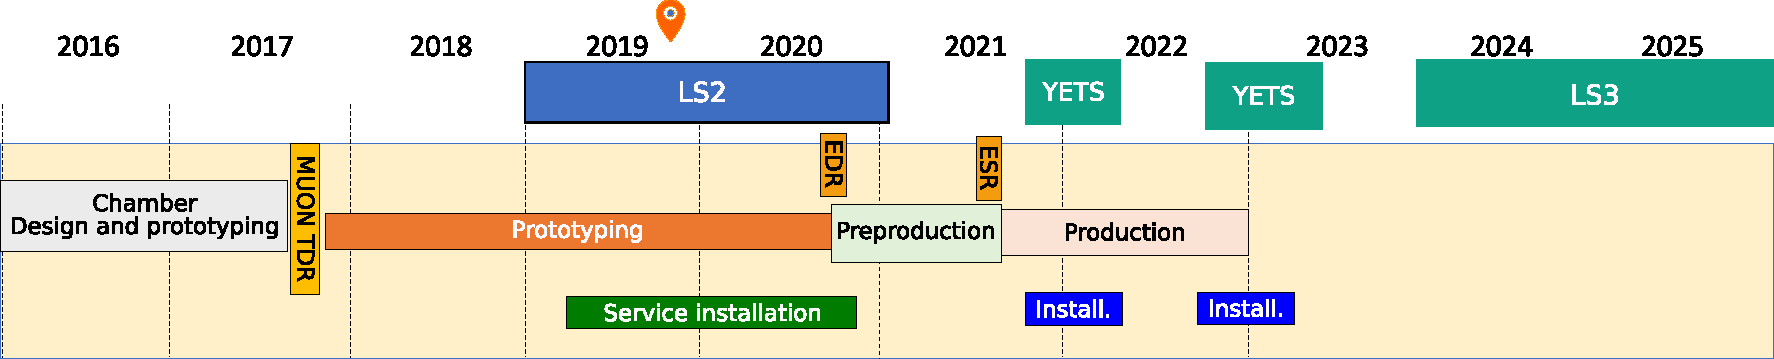
\includegraphics[width=\linewidth]{fig/chapt7/CMS-RPC-Milestones.pdf}
	    \caption{\label{fig:milestones} RE3/1 and RE4/1 prototyping and production schedule.}
	\end{figure}
	
	After LS3, the LHC will finally enter its high-luminosity phase, and new breakthroughs will be foreseen. The good performance of the RPCs and of all of the CMS sub-systems will be important in this regard and the skills developed during the present R\&D will become an important asset in maintaining the performance of the detectors at their best level.

\clearpage{\pagestyle{empty}\cleardoublepage}